\documentclass[12pt]{ociamthesis}  % default square logo 
%\documentclass[12pt,beltcrest]{ociamthesis} % use old belt crest logo
%|\documentclass[12pt,shieldcrest]{ociamthesis} % use older shield crest logo

%load any additional packages
\usepackage{amssymb}
\usepackage{amsmath}
\usepackage{url}
\usepackage[toc,page]{appendix}
\usepackage{graphicx}
\graphicspath{{./figures/}}
\DeclareGraphicsExtensions{.pdf,.png, .gif, .jpg}
\usepackage{qtree}
\usepackage{forest}
\usepackage{makecell}
\usepackage{xcolor}
\usepackage{fixltx2e}

%============ BIBLIOGRAPHY AND REFS PACKAGES ========%
\usepackage{multibib}
\newcites{x}{References}
\newcites{sec}{Background Reading}

%============ for gloss overline ========%
\makeatletter
\newcommand{\OVER}[1]{$\overline{\hbox{#1}}\m@th$}
\makeatother

\newcommand{\TAG}{\textsuperscript}
\newcommand{\SUB}{\textsubscript}

% ============== stuff below is for header\footer
\usepackage{fancyhdr}
\pagestyle{fancy}
\fancyhead{}
\renewcommand{\sectionmark}[1]{\markright{\textit{#1}}}
\renewcommand{\chaptermark}[1]{\markboth{\textsc{#1}}{}}
%\fancyhead[LO]{\leftmark}
%\fancyhead[RE]{\rightmark}
\fancyhead[R]{\rightmark}
\fancyhead[L]{\leftmark}
\cfoot{\fancyplain{}{\thepage}}

% ============== FRONT PAGE =========== %
        
\title{Automated Visualised Translation from English to British Sign Language}

\author{Nicolaos Moscholios}             %your name
\college{Pembroke College}  %your college

\degree{Master of Computer Science}     %the degree
\degreedate{Trinity 2016}         %the degree date

%end the preamble and start the document
\begin{document}

%this baselineskip gives sufficient line spacing for an examiner to easily
%markup the thesis with comments
\baselineskip=18pt plus1pt

\maketitle                  % create a title page from the preamble info

\begin{abstract}
A large number of people in the world today are born deaf and many rely on British Sign Language (BSL), the most widely used method of signed communication in the UK. BSL is structured in a completely different way to English and, like any language, it has its own grammar. In order to create a communication bridge between English speakers and individuals affected by deafness there have been attempts at building a formal model of translation. ...
\end{abstract}

\begin{acknowledgements}
I would like to thank...
\end{acknowledgements}

\begin{notes}
The work described in this thesis is available online at \url{nicmosc.com/bsltranslate}. Examples discussed throughout the report marked by an asterisk ($\ast$) can be viewed on the website. For demonstrative purposes it is highly suggested that the Examiner try those examples ..
\end{notes}

%\include{abstract}          % include the abstract
{\pagestyle{plain}
	\begin{romanpages}          % start roman page numbering
	%set the number of sectioning levels that get number and appear in the contents
	\setcounter{tocdepth}{5}
	\setcounter{secnumdepth}{5}
	\tableofcontents            % generate and include a table of contents
	\listoffigures              % generate and include a list of figures
	\listoftables
	\end{romanpages}            % end roman page numbering
\cleardoublepage}

%===================== CHAPTER 1 ===================%

\chapter{Introduction}
For most people around the world, communication is achieved orally by speaking. Unfortunately some are born deaf or are affected by hearing impairment with time. It is then necessary to use another medium of communication. Today there are about 1 million "functionally deaf" UK individuals \citex{website:bsl-stats}, that is, that require the use of sign language to converse. Additionally there are around 11 million people affected by some degree of hearing loss and while many benefit from hearing aids, sign language bypasses the need to speak, making it easy for everyone to understand each other.  

\section{Motivation}
The problem arises when hearing and Deaf individuals need to communicate. Deaf individuals are taught to read and write English from a young age, but it was found that they have difficulties understanding text with a reading level above that of primary school students \citex{paper:deaf-edu}. Thus it is not enough for hearing individuals to rely on written text to communicate with their community. More and more people are learning BSL even though they have perfectly fine hearing. There are certificates that can be obtained to work with Deaf individuals \citex{website:signature}. Taking lessons from BSL teachers and practising with the community helps to learn the language.

Online resources such as UCL's BSL Sign Bank \citex{website:bsl-sign-bank} and SignBSL.com \citex{website:sign-bsl} offer clips of signers showing words and phrases in BSL for learners and curious people?. The main issue is that they are highly static. Analogously to an English dictionary, it is only useful for looking up individual signs and not \textit{translating} phrases. Automated translation has been an ongoing challenge in the field of
computational linguistics, and we are finally seeing very positive results thanks to the recent developments in machine learning. Since spoken (written) languages are heavily dependent on their syntactic components, they are relatively easy to formalise in such a way that a machine can interpret a sentence and perform operations on it to transition from one language to another. More recently, there have also been attempts at doing so with signed languages such as ASL (American Sign Language) and BSL. Given that there is no formally typed grammar for BSL, it is not easy to find a model that encapsulates all key elements involved, such as facial expressions and eye gaze. In addition, since the language is only signed, the only way to see if an interpretation is correct, is through visual output. While some past implementations have been successful, due to the then high computational power necessary to run these systems, most of them are now outdated or have been left at a prototype stage. In 2006, IBM created a fully working system \citex{website:IBM} that allowed users to speak and see the translation from English to BSL in real time; however it has been disregarded and is not available any more. 

\section{Objectives}
This project will build upon previous work and attempt to solve the interlingual translation from English to British Sign Language by implementing a web application where signs are visualised through a virtual avatar. Behaviour will closely follow that of other established translation systems such as Google Translate where users can type a sentence and get a result in real-time. Through rule-based translation methods (discussed in section \ref{machine translation}) and 3D animation techniques the system will allow users to not only find out what a particular sentence corresponds to in BSL, but also learn and hopefully practice their skills. Figure \ref{fig:sys-overview} shows a conceptual overview of the system pipeline; this figure will be references multiple times throughout the report.

\begin{figure}[h]
	\centering
    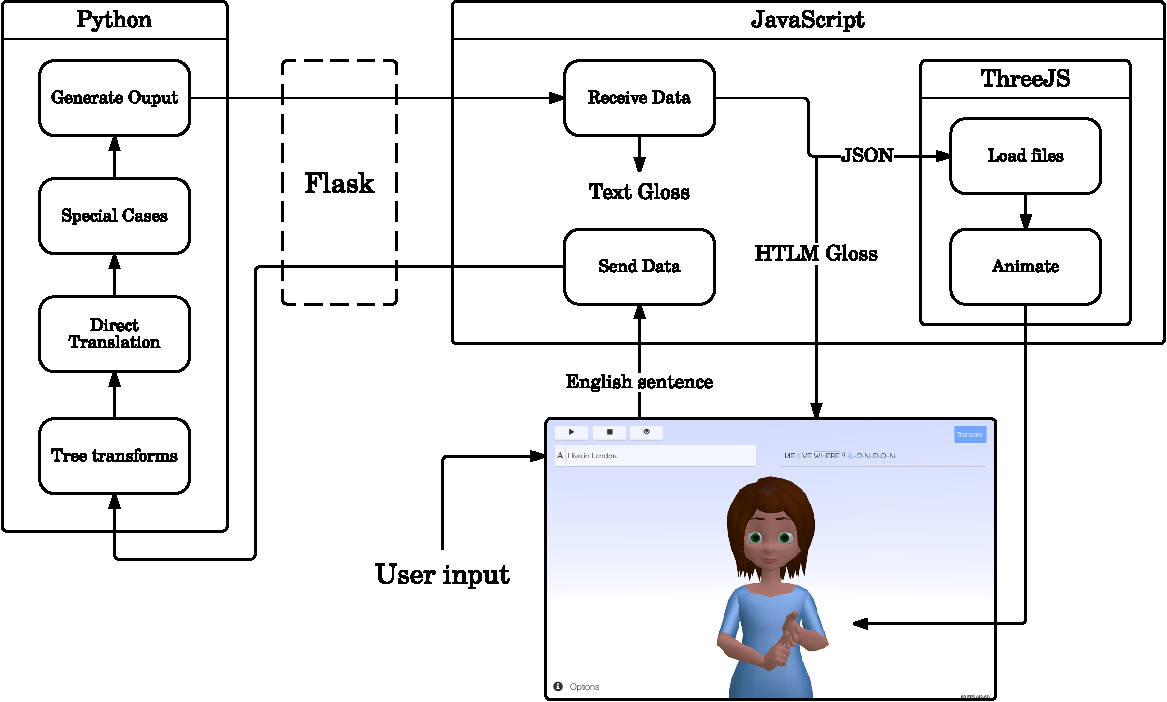
\includegraphics[scale=0.75]{system-overview}
    \caption{Conceptual overview of the system}
    \label{fig:sys-overview}
\end{figure}

\section{Structure}
The report will read as follows: in chapter 2 we will give a brief introduction to the linguistics British Sign Language and its differences from written English, as well as existing methods of translation from written to written and from written to signed languages. Chapter 3 will cover the design choices for the system, that is, the development environment with the programming languages, the conceptual structure of the pipeline and the end-user interaction. Following up in chapter 4 we explain in detail the implementation of both the translation methods and the animation techniques utilised, as well as the communication between the two modules. Finally chapter 5 will discuss the evaluation of the system both in terms of translation accuracy and feedback from the user survey, while chapter 6 concludes the report along with project achievements, personal remarks and future work.

%===================== CHAPTER 2 ===================%

\chapter{Background}
\section{British Sign Language: Linguistics Overview}
This section will give a short introduction to the linguistics of British Sign Language, including common grammar rules, its morphology and how it differs from written English. Please note that only the most general information is described here, that is enough to follow concepts described in section \ref{existing methods} and the implementation of the system (chapter \ref{implementation}). The following examples and explanations are based on the book by Woll and Sutton, \textit{The Linguistics of British Sign Language: an Introduction}.

British Sign Language, often shortened to BSL, has been an officially recognised language since 2003 \citex{website:signature}. Like English, it has its own grammar \citex{website:deafness} and its own lexicon. While not as large as its written counterpart, there are enough signs to convey the same ideas in sign language, as many can be combined (\textit{compounds}, see section \ref{morphology}) to create new meanings. However BSL is not the only signed language; each country has their own with different dialects by region. ...  

Talk about non-manual features here

Since BSL can only be transmitted through signing, there is no formal written form. Many different formats exist such as Stokoe, designed for ASL by William Stokoe only for representing hand movements \citex{paper:stokoe} (thus carries no information about non-manual features) later adapted to BSL by Kyle and Woll \citex{book:bsl-stokoe}, HamNoSys (Hamburg Notation System) that can represent any signed language \citex{paper:hamnosys}, SignWriting which uses visual icons to represent parts of the body \citex{thesis:signwrite} and more. The most commonly used method to represent sign language without needing to learn the notation (all of the above require additional knowledge to be decoded) is through \textit{gloss}. Gloss uses the most basic representation of the sign in its English written form. For example if one wants to describe a situation where a girl is eating an apple, the gloss would be GIRL EAT APPLE. The advantage of this notation is that we can clearly understand what a sentence means as we associate the sign to its English meaning. The main disadvantage though is that there is no information about the sign whatsoever, we only know that the particular sign for GIRL is signed first, followed by the sign for APPLE and so on. Table \ref{table:comparison} shows an example sign for every notation type.

Gloss notation also carries some information about non-manual features, for example the sentence ``Where do you live?'' would be YOU LIVE \OVER{WHERE }\TAG{br}, where br represents a brow raise for asking questions. ?This is the format we will use for the rest of the report and it is what is used in the application as well?.

\begin{table}[ht]
\begin{center}
\begin{tabular}{| c | c | c | c | c | c |}
	\hline
	English & Sign & SignWrite & Stokoe & HamNoSys & Gloss \\ \hline
	\Large What? & \raisebox{-.5\height}{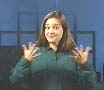
\includegraphics[scale=0.8]{chapter2/woman}}
    & \raisebox{-.5\height}{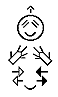
\includegraphics[scale=0.7]{chapter2/signwrite}}
    & \raisebox{-.5\height}{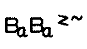
\includegraphics[scale=0.6]{chapter2/stokoe}}
    & \raisebox{-.5\height}{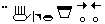
\includegraphics[scale=0.8]{chapter2/ham}}
    & \OVER{WHAT }\TAG{br}
    \\ \hline
\end{tabular}
\caption{Examples of different BSL written forms}
\label{table:comparison}
\end{center}
\end{table}

\subsection{Structure of sentences}
In English, sentences often follow very similar patterns. Most often we find a noun phrase followed by a verb phrase, each one containing information about the subject and the object\ref{fig:english-sent}. BSL borrows some elements from English, such as the concept of pronouns, adjectives, verbs etc. but also includes \textit{proforms} and \textit{classifier predicates} which do not exist in English. -

\begin{figure}[h]
\Tree [.S
 	   	 [.NP 
			[.\textcolor{red}{DT} The ] 
			[.\textcolor{red}{JJ} large ] 
			[.\textcolor{red}{NN} cat ] 
 	   	 ]
 	   	 [.VP 
 	   	 	[.\textcolor{red}{VBP} sat ] 
			[.PP 
				[.\textcolor{red}{IN} on ]
				[.NP 
					[.\textcolor{red}{DT} the ] 	
					[.\textcolor{red}{NN} mat ] 			
				]		
			] 	   	 
 	   	 ]
 	 ]
\caption{English sentence syntax tree}
\label{fig:english-sent}
\end{figure}

In word order: mention that we can use SVO although some verbs require SOV like ME PIZZA EAT (eat is modified by the type of object we are eating)

\subsection{Morphology and Morphemes}
\label{morphology}
A morpheme in BSL is considered as the smallest unit of meaning in a word or sign. We can combine them to form signs that have several meaningful parts but are still considered a single sign. Figure \ref{fig:morphemes} shows the BSL sign morphology tree. We distinguish between \textit{monomorphemic} signs (cannot be further subdivided) like TRUE, SAY, MOUSE and \textit{polymorphemic} which are a combination of 2 or more morphemes. For example PROMISE is the combination of the sign for SAY and TRUE, or CHECK = SEE + MAYBE. We also categorise morphemes as \textbf{Free} that can stand alone (i.e. monomorphemes like RED, TRUE, SAY) and \textbf{Bound} which have a meaning but \textit{must} be combined with at least one other morpheme, and \textbf{Plural} morphemes.  

\begin{figure}[h]
\begin{forest}
[Signs
	[\makecell{Monomorphemic \\ (free morphemes)}]
    [Polymorphemic 
		[\makecell{2 (or more) free \\ morphemes "compounds"}] 
		[\makecell{Combination of bound \\ and free morphemes}] 
		[\makecell{Combination of 2 \\ (or more) bound morphemes}]
	]
]
\end{forest}
\caption{BSL sign morphology schema}
\label{fig:morphemes}
\end{figure}

Free morphemes are often combined to form a \textbf{compound}, a sign with a different but related meaning. Some are borrowed from English like BALANCE-SHEET while others aren't: BLOOD = RED + FLOW, TIGER = ZEBRA + ANIMAL. When combining free morphemes, the compound must appear as similar as possible to a single sign, thus the originals are modified by rapid transitioning (both signs are accelerated), the initial hold of the first sign and any repeated movement in the second sign are lost. For example if MOTHER = -M-M- and FATHER = -F-F- then PARENTS = -M-F- and not -M-M-F-F-.

Bound morphemes must be attached to another free morpheme. The sign for DRIVE-CASUALLY combines the free morpheme DRIVE (verb) and bound CASUALLY, since we need to specify what action is being performed in a casual manner. Similarly the agreement verb ASK (see section \ref{verbs}) requires the subject and object such as YOU and ME (both free morphemes) to form the complete verb YOU-ASK-ME.

Plural morphemes include both free and bound morphemes and can carry information about nouns and verbs. In English this trait corresponds to the terminal \textit{-s}. In ``cats'' we find cat + s where [s] is the form of a \textit{bound} morpheme: it cannot stand alone. However in BSL we cannot just add a terminal to the sign. Instead plural morphemes can be attached to a sign, modify the sign itself or appear separately. For example the plural ``children'' can be signed as CHILD repeated multiple times, or we can  sign TWO CHILD if we know there are 2 of them, or otherwise using pronouns like CHILD THEM to mean that there are more than one.

Adjectives also carry some morphological information as they convey a particular feature of nouns or pronouns. Adjectives can be \textbf{attributive} when they occur in the noun phrase and appear before, after or within a noun e.g. SHIRT WHITE, or \textbf{predicative} when they act like a verb e.g. MAN Index\textsubscript{3} TALL where the man is ``executing'' the action of being tall. However they are not used very often, since signs can be modified directly instead; the sign for BOX involves making a square shape with both hands, however SMALL-BOX and LARGE-BOX will modify the movement for the base sign by leaving less or more space between the hands respectively. Signs that cannot be directly modified make use of the normal adjective signs (there is indeed a sign for both small and large) and can be preceded by a premodifier like VERY, QUITE etc. Adjective signs in comparative (\textit{-er}) and superlative (\textit{-est}) form are modified by making the initial hold very long and tense, followed by a rapid release, where the degree of tension depends on the modifier.

\subsection{Verbs}
\subsubsection{Tense, Aspect and Manner}
In English when we want to refer to an action that will happen in another point in time we conjugate the verb (``He will go home'') or use words that convey the same idea (``He's going home tomorrow''). BSL uses WILL and TOMORROW as keywords to show an action happening at a different time.

All of the above are normally passed through adverbs in English, while in BSL they are incorporated into the verbs themselves.
\subsubsection{Verb types}
\label{verbs}
Topographic vs. Syntactic space, plain, agreement, spatial verbs

\subsection{Questions and Negations}
\label{qneg}
When asking a question, the whole sentence is accompanied by a brow raise, a head tilt and opened eyes. The question ``Do you like tea?'' is \OVER{YOU LIKE TEA }\TAG{q}. Some questions only include a brow raise on parts of the sentence, such as in ``You have three children right?'' = THREE CHILD HAVE \OVER{RIGHT}\TAG{q} since we are asking for confirmation.

Wh- question, which include \textit{what, why, where, when, who, which, how} usually follow the same rule as the above where only the wh- word is accompanied by a question facial expression. For example:
\begin{flalign*}
&\text{Who are your parents?} = \text{YOUR -M-F- \OVER{WHO }\TAG{q}} \tag{$\ast$} \\
&\text{Where did he go?} = \text{Index\SUB{1} GO \OVER{WHERE }\TAG{q}} \tag{$\ast$}
\end{flalign*}
However questions can also be used in sentences which are not questions by nature. In fact the following
\begin{flalign*}\tag{$\ast$}
&\text{I love John because he's nice} = \text{ME LOVE -J-O-H-N- \OVER{WHY }\TAG{q} Index\SUB{1} NICE} \\
&\text{I won't go to the beach if it'll rain tomorrow} \\
&= \text{\OVER{TOMORROW RAIN}\TAG{q} ME \OVER{NOT GO }\TAG{neg} BEACH} \tag{$\ast$}
\end{flalign*}
essentially turning the sentence into a rhethorical question. The same happens when we try to describe the state of an object or person like
\begin{flalign*}
&\text{The keys are in the kitchen} = \text{KEYS \OVER{WHERE }\TAG{q} KITCHEN} \\
&\text{I live in Oxford} = \text{ME LIVE \OVER{WHERE }\TAG{q} -O-X-F-O-R-D} \tag{$\ast$}
\end{flalign*}

Sentences that contain negations are signed considering three main elements: \\
\textbf{Facial expression}: the lips are pushed out and the eyes are narrowed \\
\textbf{Head movements}: the head turns to the side and is held there (accompanies a specific sign) or alternates between the left and right sides. The latter can negate both whole sentences or single signs e.g.
\begin{flalign*}
\text{I'm not eating pizza} = & \text{\OVER{ME PIZZA EAT }\TAG{neg}} \\
&\text{ME PIZZA \OVER{EAT }\TAG{neg}} \\
&\text{ME PIZZA EAT \TAG{neg} }
\end{flalign*}
\textbf{Negation signs}: these are specific hand gestures to show that a negation is happening, the most common ones are a flat hand, palm down twisting up following a verb or adjective (often used as a suffix with SEE+neg, HAVE+neg for denial of possession or experience) and the NOT sign. Thus the previous example can also be written as
\begin{flalign*}
\text{I'm not eating pizza} = & \text{ME PIZZA \OVER{NOT EAT}\TAG{neg}}
\end{flalign*}
Additionally, some signs when negated are completely different from the original and are not just preceded by NOT and the \textit{neg} expression. For example the verb ``know'' is performed by the dominant hand's fist with the thumb up tapping on the forehead, while its negation NOT-KNOW sees the two flat hands moving away from the forehead.

\subsection{Fingerspelling}
Fingerspelling is the action of using the signed alphabet to spell out a word, normally borrowed from English. The most general rule for figerspelling is that if the word is less than 3-4 letters long it is spelled in full, otherwise it can be abbreviated. The fingerspelling notation in gloss form is -B-B-C or -b-b-c- (example for the commonly known broadcasting company). There exist a few abbreviation rules however the most common ones are:
\begin{itemize}
	\item Using the first syllable e.g. January = -J-A-N-
	\item When the second letter is `h' we retain the first 2 e.g. chapter = -C-H-
	\item We can also use the first and last letter (mainly used for places) e.g. Glasgow = -G-W-
\end{itemize}
However if an unknown word is introduced in a context for the first time, such as personal name or a place name, then it is first spelled in full, and the following time the abbreviation is used. The name Hannah may be signed as -H-A-N-N-A-H- first and then just as -H-. On the other hand it is not uncommon for signers to use body/character features to refer to someone. For example if I would like to talk about a person that wears glasses, I would first need to sign their full name, followed by the sign for glasses. After setting that context the listener would know that every time GLASSES is signed, that person is being referred to.

\subsection{Non-manual features}
Non-manual features represent any action performed by the signer which is not performed by the hands and are used to represent spoken language mouth patterns in combination with signs, enacting actions and setting the context like verb tenses and questions. These are very important in BSL and are often mistakenly neglected by (in common knowledge/culture??)
\subsubsection{Spoken and Oral Components}
Spoken components are used to better identify the sign being used. Nouns that are fingerspelled are also mouthed when the last letter is signed; this also applies to abbreviated signs i.e. only one letter is signed but the whole word is mouthed. They are also extremely useful with homonyms, since only through mouthing it is possible to distinguish two meanings of a sign that has the same gestures e.g. FINLAND and METAL. The mouthing shape is borrowed from the English spoken version of the words.

Oral components enact real-life actions such as laughing or biting, where the sign is entirely mouthed (the hands are not involved, although there are manual versions of such actions as well). Additionally, mouthing can be used to represent negations as described in section \ref{qneg}.
\subsubsection{Facial Expressions and Head Movements}
Facial expressions are used to mark a question (as seen above), to show emotions e.g.
\begin{flalign*}
\text{I was happy when dad arrived} = & \text{\OVER{ME HAPPY }\TAG{happy} WHEN -D-D- ARRIVE}
\end{flalign*}
They are also used in combination with a head nod to mark the topic. The topic can be \textit{temporal} when describing a situation in time such as ``When I$\ldots$'', \textit{spatial} and \textit{nominal} when describing a location or an entity. Most often said entity is the subject of the sentence thus
\begin{flalign*}
\text{The dog chased the cat} = & \text{\OVER{DOG }\TAG{hn} CAT CHASE}
\end{flalign*}
where hn stands for head nod.

\subsubsection{Eye Gaze}
\label{eye-gaze}

\section{Online Resources}

\section{Machine Translation}
\label{machine translation}
\subsection{Classical}
\subsection{Statistical}

\section{Existing Methods}
\label{existing methods}
\section{Personal Work}
\section{Summary}

%===================== CHAPTER 3 ===================%

\chapter{Design}

\section{Language Choice}
\section{Translation}
\section{User Interface}
	\subsection{User Interaction}
\section{Summary}

%===================== CHAPTER 4 ===================%

\chapter{Implementation}
\label{implementation}

\section{Rule-Based MT in Python}
	\subsection{Pipeline}
	\subsection{System Components}
		\subsubsection{Grammar Tree Transforms}
		\subsubsection{Direct Translation}
		\subsubsection{Special Cases}
		\subsubsection{Output}
	
\section{Animation in ThreeJS}
	\subsection{Blender}
		\subsubsection{Model}
		\subsubsection{Skeletal Animation}
	\subsection{Data Format}
		\subsubsection{JSON Formatter}
	\subsection{Animation Engine}
		\subsubsection{Pipeline}
		\subsubsection{ThreeJS}
	
\section{Interlingual Communication with Flask}
	\subsection{Python to JavaScript}

\section{Summary}
			
%===================== CHAPTER 5 ===================%

\chapter{Evaluation}

\section{Translation}
	\subsection{BLEU}
\section{Animation}
\section{Survey}
\section{Feedback}

%===================== CHAPTER 6 ===================%

\chapter{Conclusion}

\section{Improvements}
	\subsection{Handling of Agreement Verbs}
	\subsection{Classifiers}
\section{Expansion}

%===================== APPENDIX ===================%

%now enable appendix numbering format and include any appendices
{\pagestyle{plain}
\appendix
\chapter{Extra code (appendix)}

%===================== REFREENCES ===================%
%next line adds the Bibliography to the contents page
\addcontentsline{toc}{chapter}{References}
\bibliographystylex{plainurl}
\bibliographyx{references.bib}
\newpage

\addcontentsline{toc}{chapter}{Background Reading}
\nocitesec{*}
\makeatletter
\renewcommand\@biblabel[1]{}
\makeatother
\bibliographystylesec{plainurl}
\bibliographysec{bibliography.bib}
\cleardoublepage}

\end{document}